\documentclass[12pt]{article}

\usepackage[a4paper,margin=2cm]{geometry}

\usepackage{amsmath}
\usepackage{amssymb}
\usepackage{mathtools}

\usepackage{listings}

\usepackage{booktabs} % For tables
\usepackage[table,xcdraw]{xcolor} % For tables

\usepackage{tikz} % TikZ

\usepackage{enumerate}
\usepackage{enumitem}

\usepackage{nameref}

\usepackage{xcolor}

\definecolor{codegreen}{rgb}{0,0.6,0}
\definecolor{codegray}{rgb}{0.5,0.5,0.5}
\definecolor{codepurple}{rgb}{0.58,0,0.82}
\definecolor{backcolour}{rgb}{0.95,0.95,0.92}

\lstdefinestyle{mystyle}{
    backgroundcolor=\color{backcolour},
    commentstyle=\color{codegreen},
    keywordstyle=\color{magenta},
    numberstyle=\tiny\color{codegray},
    stringstyle=\color{codepurple},
    basicstyle=\ttfamily\footnotesize,
    breakatwhitespace=false,
    breaklines=true,
    captionpos=b,
    keepspaces=true,
    numbers=left,
    numbersep=5pt,
    showspaces=false,
    showstringspaces=false,
    showtabs=false,
    tabsize=2
}

\lstset{style=mystyle}

\DeclarePairedDelimiter\abs{\lvert}{\rvert}
\DeclarePairedDelimiter\Abs{\lVert}{\rVert}

\usepackage{fancyhdr}

\pagestyle{fancy}
\lhead{\today}
\chead{Exercise 04\\Algorithmic Foundations of Data Science}
\rhead{Fabian Grob\\Simon Michau\\Til Mohr}

\setlength{\headheight}{50pt}

\begin{document}

\section*{Exercise 1}
\subsection*{(a)}
Situation for l=2 and s=2:
\[Q_{2,2}=\lbrace [x_1 x_2]^T\in\mathbb{R}^2\mid |x_i|\leq 1 \text{ for all } i=1,2\rbrace = [-1,1]^2\]
\begin{center}
	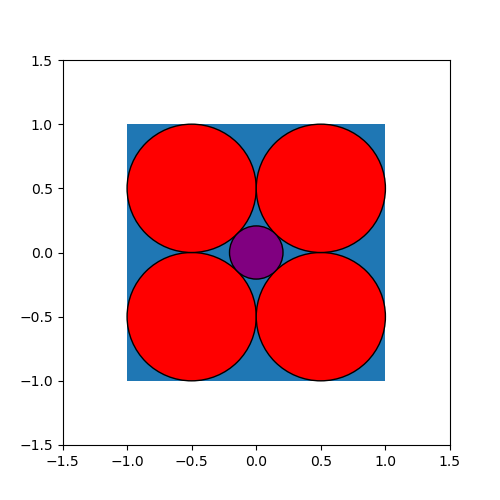
\includegraphics[width=3.5in]{code/exercise_01_a.png}
\end{center}

\subsection*{(b)}
First, let's calculate the radius of the inner hyperball for any $l \in \mathbb{N}, s \in \mathbb{R}_{>0}$: \\
The distance from the center of the inner hyperball (equal to the center of the hypercube) to the center of one of the $2^l$ outter hyperballs (doesn't matter which one) can be calculated the following:
\begin{equation*}
	d \coloneqq \sqrt{l \cdot \left( \frac{s}{4} \right)^2}
\end{equation*}
Thus, the radius of the inner hyperball is equal to:
\begin{equation*}
	r \coloneqq d - \frac{s}{4} = \sqrt{l \cdot \left( \frac{s}{4} \right)^2} - \frac{s}{4}
\end{equation*}
Now, we simply must solve the following inequality to find an $l \in \mathbb{N}$ for an arbitrary but fixed $s \in \mathbb{R}_{>0}$ such that $B(Q_{l,s}) \not\subseteq Q_{l,s}$:
\begin{align*}
	\frac{s}{2} &< r \\
	\frac{s}{2} &< d - \frac{s}{4} \\
	\frac{s}{2} &< \sqrt{l \cdot \left( \frac{s}{4} \right)^2} - \frac{s}{4} \\
	\frac{3 \cdot s}{4} &< \sqrt{l} \cdot \frac{s}{4} \\
	3 &< \sqrt{l} \\
	l &> 9
\end{align*}

\section*{Exercise 2}
\subsection*{(a)}
Let's first find all eigenvalues of $A_c$:
\begin{align*}
	\{ \lambda \in \mathbb{R} &\mid \det\left( A_c - \lambda \cdot I_3 \right) = 0\} \\
	\{ \lambda \in \mathbb{R} &\mid \det\left[ \begin{array}{ccc} 2 - \lambda & 0 & c \\ 0 & 1 - \lambda & 0 \\ c & 0 & 1 - \lambda \end{array} \right] = 0\} \\
	\{ \lambda \in \mathbb{R} &\mid -\lambda^3 + 4 \cdot \lambda^2 + c^2 \cdot \lambda - 5 \cdot \lambda + 2 -c^2\} \\
	\{ \lambda \in \mathbb{R} &\mid (\lambda - 1) \cdot (-\lambda^2 + 3 \dot \lambda + c^2 - 2)\} \\
	\{ 1, \frac{3 - \sqrt{4 \cdot c^2 + 1}}{2}, \frac{3 + \sqrt{4 \cdot c^2 + 1}}{2}\} \eqqcolon \Lambda_{A_c}\\
\end{align*}
So, if for all $\lambda \in \Lambda_{A_c}$ it must hold that $\lambda \geq 0$, we must set $c$ such that the following inequality holds:
\begin{align*}
	\frac{3 - \sqrt{4 \cdot c^2 + 1}}{2} &\geq 0 \\
	3 - \sqrt{4 \cdot c^2 + 1} &\geq 0 \\
	3 &\geq \sqrt{4 \cdot c^2 + 1} \\
	9 &\geq 4 \cdot c^2 + 1 \\
	8 &\geq 4 \cdot c^2 \\
	2 &\geq c^2 \\
	c \in (-\sqrt{2}&, \sqrt{2}) \subseteq \mathbb{R}
\end{align*}

\subsection*{(b)}
Using Theorem 5.19, we create an orthogonal matrix $U \in \mathbb{R}^{3 \times 3}$ with the columns being the eigenvectors of $A$. We can now use Theorem 5.20 to create the diagonal matrix $\Lambda \in \mathbb{R}^{3 \times 3}$ where the eigenvalue-entry $\lambda_{i,i}$ corresponds to eigenvector in the column $i$ of $U$. \\
A simple verification:
\begin{align*}
	A &= U \Lambda U^\top \\
	A &= U \Lambda U^{-1} \\
	A U &= U \Lambda \\
	A v_i &= v_i \lambda_{i,i} \qquad, \forall i \in \left[3\right], v_i \coloneqq col_i(U) \\
	A v_i &= \lambda_{i,i} v_i \qquad, \forall i \in \left[3\right], v_i \coloneqq col_i(U) \\
\end{align*}
Since $A$ is positive semi-definite, all entries $\lambda_{i,i} \geq 0$. Thus, we can create a diagonal matrix $\Lambda'$ consisting of the entries $\lambda'_{i,i} \coloneqq \sqrt{\lambda_{i,i}}$. Thus, $\Lambda = \Lambda' \Lambda'^\top$. Let $B \coloneqq U U \Lambda'$. Now:
\begin{align*}
	A &= U \Lambda U^\top \\
	A &= U (\Lambda' \Lambda'^\top) U^\top \\
	A &= U (\Lambda' \Lambda'^\top) U^\top \\
	A &= (U \Lambda') (\Lambda'^\top U^\top) \\
	A &= (U \Lambda') (U \Lambda')^\top \\
	A &= B B^\top \\
\end{align*}

\subsection*{(c)}

\section*{Exercise 3}
\subsection*{(a)}
\subsection*{(b)}
\subsection*{(c)}
\subsection*{(d)}

\section*{Exercise 4}
\subsection*{(a)}
\subsection*{(b)}
\subsection*{(c)}
\subsection*{(d)}
\subsection*{(e)}

\section*{Exercise 5}


\end{document}
